Our robot Dora is a Pioneer 3D-X differential robot platform with an in-house central supporting construction attached to it. This construction serves as support for the various sensors and the laptop which is the brain of the robot (see Fig~\ref{fig:dora}). In terms of sensing Dora is equipped with 2 laser rangefinders and 1 depth camera. These sensors are primarily used to ensure safe navigation 
and people detection. Additionally, Dora is equipped with a microphone and speakers in order to enable  Human-Robot-Interaction and to be able to participate in the tasks involving speech.

 
\begin{figure}[!htb]
\centering
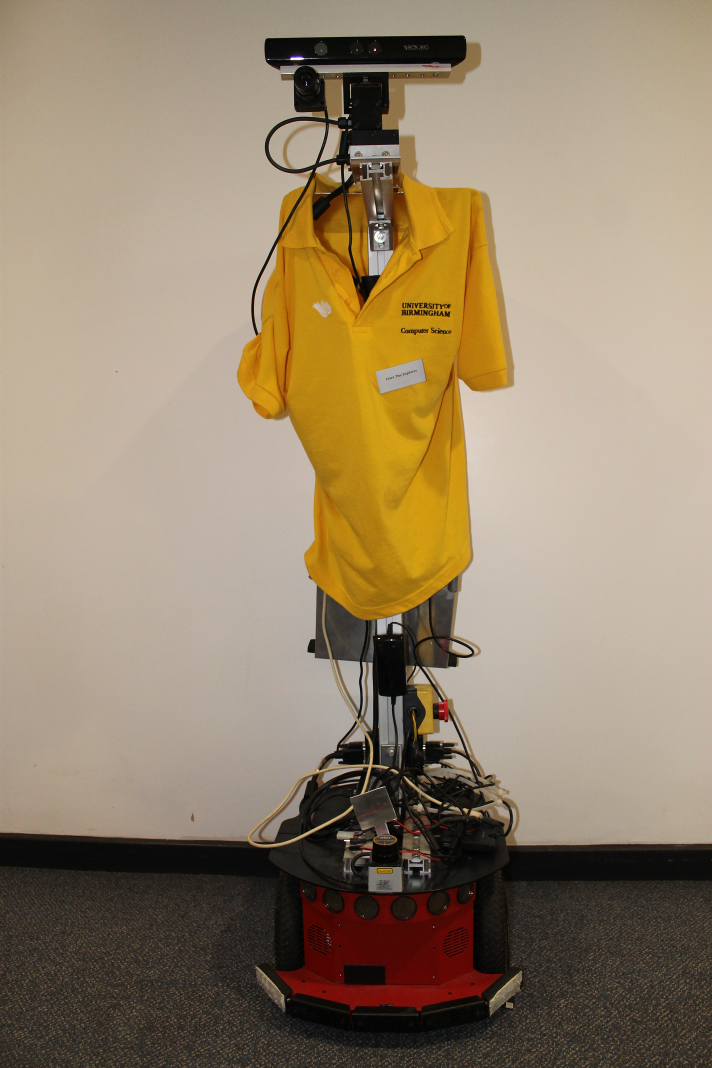
\includegraphics[width=2.in]{dora_new.png}
\caption{Dora is an extended Pioneer 3D-X robot with sensors such as laser range finders, depth cameras and a laptop mounted on top.}
\label{fig:dora}
\end{figure}  


